\documentclass[a4paper,14pt]{article}
\usepackage{float}
\usepackage{extsizes}
\usepackage{amsmath}
\usepackage{amssymb}
\everymath{\displaystyle}
\usepackage{geometry}
\usepackage{fancyhdr}
\usepackage{multicol}
\usepackage{graphicx}
\usepackage[brazil]{babel}
\usepackage[shortlabels]{enumitem}
\usepackage{cancel}
\usepackage{textcomp}
\usepackage{array} % Para melhor formatação de tabelas
\usepackage{longtable}
\usepackage{booktabs}  % Para linhas horizontais mais bonitas
\usepackage{float}   % Para usar o modificador [H]
\usepackage{caption} % Para usar legendas em tabelas

\columnsep=2cm
\hoffset=0cm
\textwidth=8cm
\setlength{\columnseprule}{.1pt}
\setlength{\columnsep}{2cm}
\renewcommand{\headrulewidth}{0pt}
\geometry{top=1in, bottom=1in, left=0.7in, right=0.5in}

\pagestyle{fancy}
\fancyhf{}
\fancyfoot[C]{\thepage}

\begin{document}
	
	\noindent\textbf{8FMA109 - Matemática} 
	
	\begin{center}Retas secantes a uma circunferência (Versão estudante)
	\end{center}
	
	\noindent\textbf{Nome:} \underline{\hspace{10cm}}
	\noindent\textbf{Data:} \underline{\hspace{4cm}}
	
	%\section*{Questões de Matemática}	
    \begin{multicols}{2}
    	\noindent Na figura a seguir, $r$ e $x$ são secantes à circunferência, pois a interceptam em dois pontos distintos cada. É verdade que:
    	$PA \cdot PB = PC \cdot PD$ 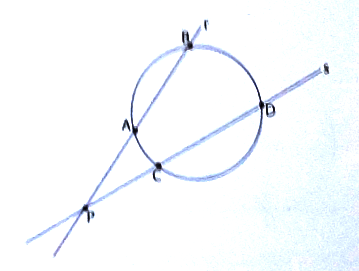
\includegraphics[width=1\linewidth]{imagens_8FMA109/imagem1}
    	
    	
    	\noindent\textsubscript{~---------------------------------------------------------------------------}
    	\begin{enumerate}
    		\item Prove a relação envolvendo as medidas de segmentos secantes à circunferência apresentada anteriormente. \\\\\\\\\\\\\\\\\\\\\\\\\\\\\\
    		\item O desenho à seguir apresenta duas semirretas de mesma origem, secantes a uma mesma circunferência.
    		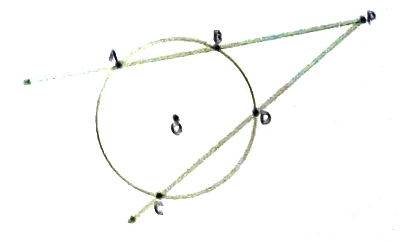
\includegraphics[width=1\linewidth]{imagens_8FMA109/imagem2}
    		
    		Calcule:
    		\begin{enumerate}[a)]
    			\item $CD$, sendo $BP$ = 5, $PD$ = 4 e $AB$ = 3. \\\\\\\\\\\\\\\\
    			\item $CD$, sendo $BP = 2AB$, $PD = \frac{PB}{3}$ e $PC = 3PA = 27.$ \\\\\\\\\\\\\\\\
    			\item Calcule os valores de $x$ nas figuras a seguir.
    			\begin{enumerate}[a)]
    				\item $~$\\
    				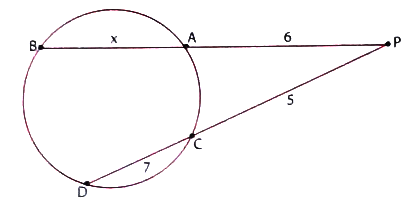
\includegraphics[width=1\linewidth]{imagens_8FMA109/imagem3} \\\\\\\\\\\\\\\\\\\\\\\\\\\\\\\\\\\\\\\\\\\\\\\\\\\\\\\\\\\\\\\\\\
    				\item $~$ \\
    				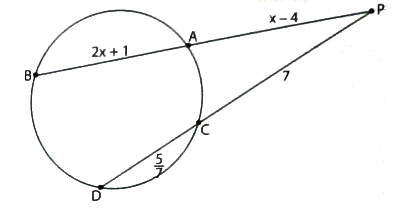
\includegraphics[width=1\linewidth]{imagens_8FMA109/imagem4}
    			\end{enumerate}
    			
    		\end{enumerate}
    	\end{enumerate}
    $~$ \\ $~$ \\ $~$ \\ $~$ \\ $~$ \\ $~$ \\ $~$ \\ $~$ \\ $~$ \\ $~$ \\ $~$ \\ $~$ \\ $~$ \\ $~$ \\ $~$ \\ $~$ \\ $~$ \\ $~$ \\ $~$ \\ $~$ \\ $~$ \\ $~$ \\ $~$ \\ $~$ \\ $~$ \\ $~$ \\ $~$ \\ $~$ \\ $~$ \\ $~$ \\ $~$ \\ $~$ \\ $~$ \\ $~$ \\ $~$  
    \end{multicols}
\end{document}